\documentclass[a4paper, 12pt]{article} % тип документа

%%%Библиотеки
%\usepackage[warn]{mathtext}	
\usepackage[T2A]{fontenc}   %Кодировка
\usepackage[utf8]{inputenc} %Кодировка исходного текста
\usepackage[english, russian]{babel} %Локализация и переносы
\usepackage{caption}
\usepackage{gensymb}
%\usepackage{listings}
\usepackage{amsmath, amsfonts, amssymb, amsthm, mathtools}
%\usepackage[warn]{mathtext}
%\usepackage[mathscr]{eucal}
%\usepackage{wasysym}
\usepackage{graphicx} %Вставка картинок правильная
%\usepackage{pgfplots}
\usepackage{indentfirst}
% \usepackage{float}    %Плавающие картинки
\usepackage{wrapfig}  %Обтекание фигур (таблиц, картинок и прочего)
\usepackage{fancyhdr}  %Загрузим пакет
%\usepackage{lscape}
%\usepackage{xcolor}
%\usepackage[normalem]{ulem}
\usepackage{geometry}

\usepackage{titlesec}
\titlelabel{\thetitle.\quad}

\usepackage{hyperref}

\newgeometry{vmargin={20mm}, hmargin={25mm, 25mm}}
%%%Конец библиотек

%%%Настройка ссылок
\hypersetup
{
	colorlinks = true,
	linkcolor  = blue,
	filecolor  = magenta,
	urlcolor   = blue
}
%%%Конец настройки ссылок


%%%Настройка колонтитулы
\pagestyle{fancy}
\fancyhead{}
\fancyhead[L]{5.10.1}
\fancyhead[R]{Таранов Александр, группа Б01-206}
\fancyfoot[C]{\thepage}
%%%конец настройки колонтитулы


\begin{document}
	
	%%%Начало титульника
	\begin{titlepage}
		
		\newpage
		\begin{center}
			\normalsize Московский физико-технический институт \\(госудраственный университет)
		\end{center}
		
		\vspace{6em}
		
		\begin{center}
			\Large Лабораторная работа по общему курсу физики\\Квантовая физика
		\end{center}
		
		\vspace{1em}
		
		\begin{center}
			\Large \textbf{Фотоэффект.}
		\end{center}
		
		\vspace{2em}
		
		\begin{center}
			\large Таранов Александр, На подсосе: Владислав Костылев \\
			Группа Б01-206
		\end{center}
		
		\vspace{\fill}
		
	\end{titlepage}
	%%%Конец Титульника
	
	
	
	%%%Настройка оглавления и нумерации страниц
	\thispagestyle{empty}
	\newpage
	\tableofcontents
	\newpage
	\setcounter{page}{1}
	%%%Настройка оглавления и нумерации страниц

	\section{Теоретическое введение}
	
	\subsection{Базовые принципы фотоэффекта}
	
	Подвергая поверхность фотокатода освещению можно обнаружить испускание электронов с поверхности катода. Данное явление называется одноквантовым фотоэлектрическим эффектом.
	Свойства фотоэффекта не имеют объяснения в рамках классической физики, но их обоснование существует в рамках квантовой физики. Для этого используется модель квантов света -- фотонов.
	
	Рассмотрим случай монохроматического излучения частотой $\omega$. При взаимодействии фотона с электроном в веществе фотон может полностью поглотиться, передав энергию электрону:
	
	\begin{equation}
		\hbar \omega = E_{max} + W,
		\label{eq:basic}
	\end{equation}
	где $W$ -- работа выхода, $E_{max}$ -- максимальная энергия, которую может приобрести электрон. 
	
	\subsection{Фотэффект в металле}

	Рассмотрим распределение фотоэлектронов по энергии в металле.
	
	Как известно, электроны в металлах могут легко перемещаться под действием электрического поля. Эти электроны являются валентными электронами металла; они слабо связаны с кристаллической решеткой. Поведение этих свободных электронов хорошо описывается моделью идеального газа.
	
	Электроны являются фермионами, имея спин $+\frac{1}{2}$. Фермионы подчиняются принципу Паули: на одно квантовое состояние приходится не более двух фермионов с противоположными спинами. Из этого следует, что в потенциальной яме, образованной металлом, все электроны не могут расположиться на дне $E = 0$: они распределятся по разрешенным уровням до некоторой энергии $E_F$ -- \textit{энергии Ферми} (см. \ref{fig:metal}). Образуется \textit{зона проводимости}.
	
	Энергия Ферми определяется концентрацией и составляет $(1\div10)$ эВ, намного превышая тепловую энергию электронов $\approx 25$ мэВ. Поэтому влиянием температурных явлений можно пренебречь.
	
	Для выхода электрону необходимо преодолеть притяжение к металлу -- совершить \textit{работу выхода}. Ее можно оценить как работу по разнесению электрона и его "изображения" на бесконечное расстояние: $W = \frac{e^2}{r_0}$.
	
	\begin{figure}[h!]
		\centering
		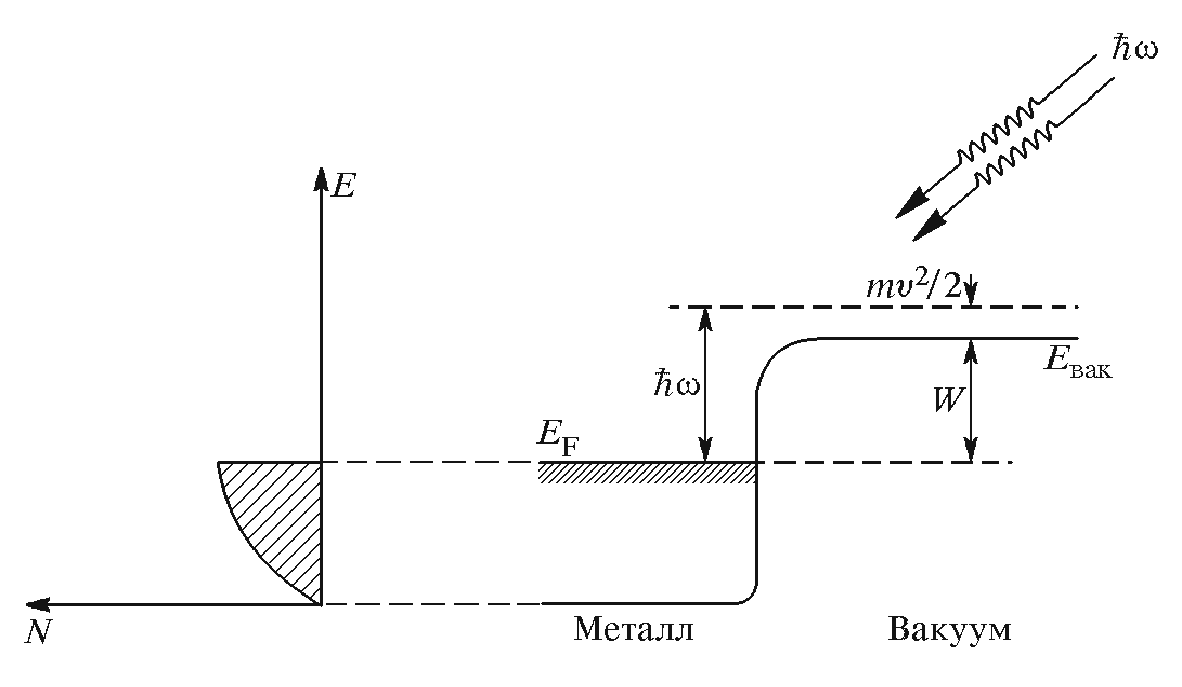
\includegraphics[scale=0.5]{res/metal.png}
		\caption{\centering
				 Модель металла как потенциальной ямы с электронным газом.
				 Слева от оси энергий: распределение электронов по энергиям.
				 Справа от оси энергий: схема зон.}
		\label{fig:metal}
	\end{figure}
	
	Таким образом, для выхода электрона из металла нужно совершить работу выхода $W$, равную разности потенциальной энергии электрона в вакууме $E_{\text{вак}}$ и энергии Ферми $E_F$. При этом фотоны, имеющие энергию $E > W$ могут выбивать электроны с более глубоких уровней. Этим объясняется распределение энергии электронов при фотоэффекте. Отметим, что квантовый выход металлов $\frac{N_{\text{электронов}}}{N_{\text{фотонов}}}$ мал, поскольку большая часть фотонов отражается.

\newpage

\subsection{Фотоэффект в полупроводниках}
	\begin{wrapfigure}[17]{l}{7.0cm}
	%                  ^^ number of occupied rows
		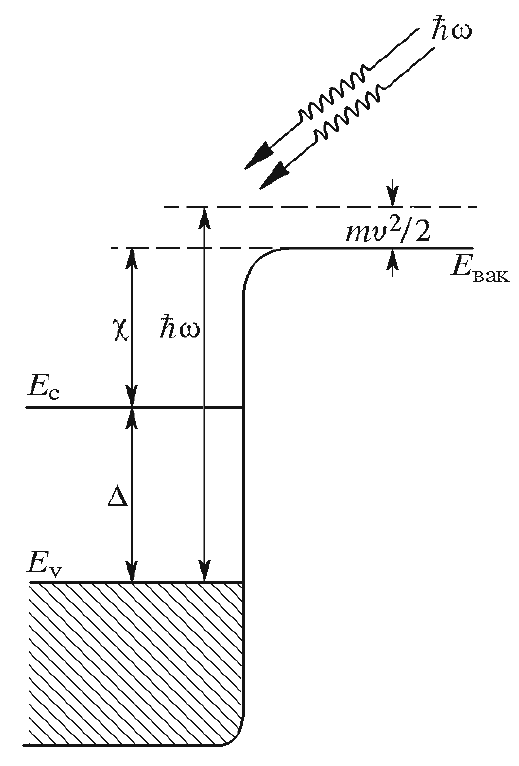
\includegraphics[scale=0.6]{res/semiconductor.png}
		% \caption{Модель полупроводника как потенциальной ямы.}
		\label{fig:semiconductor}
		\vspace{0pt}
	\end{wrapfigure}
	
	Схема зон в полупроводниках и металлах сильно различаются. В полупроводнике при абсолютном нуле валентные электроны полностью заполняют \textit{валентную зону}. Особенностью полупроводников является \textit{запрещенная зона}, которая отделяет валентную зону от зоны проводимости. Этим объясняется низкая проводимость полупроводников: проводящими являются электроны, которые попали в проводящую зону за счет тепло- или фотовозбуждения.
	
	Принципиальное описание фотоэффекта аналогично фотоэффекту в металлах, выполняется соотношение Эйнштейна: 
	
	\begin{center}
		$\hbar \omega = \Delta + \chi + E_{max}$.
	\end{center}
	
	На рис. \ref{fig:semiconductor} приведены основные обозначения, используемые для описания зон полупроводника.
	
	\begin{itemize}
		\item $E_v$ -- потолок валентной зоны,
		\item $E_c$ -- дно зоны проводимости,
		\item $E_c - E_v = \Delta$ -- ширина запрещенной зоны,
		\item $E_{\text{вак}} - E_c = \chi$ -- электронное сродство.
	\end{itemize}
	
	\newpage
		
	\subsection{Измерение энергии электронов}
	\begin{wrapfigure}{r}{7.0cm}
		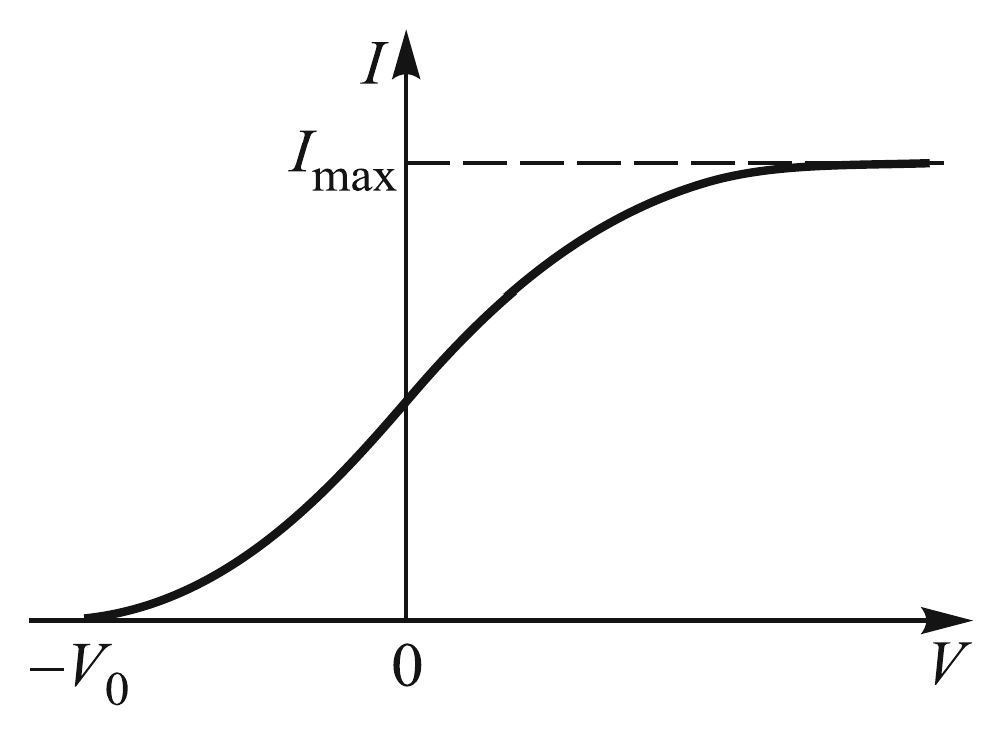
\includegraphics[scale=0.3]{res/iv_curve.png}
		\caption{ВАХ для пары фотокатод-анод.}
		\label{fig:iv_curve}
		\vspace{-10pt}
	\end{wrapfigure}

	Для измерения энергии фотоэлектронов используются пара фотокатод-анод. Между ними создается \textit{ускоряющий} $(V < 0)$ или \textit{задерживающий} $(V > 0)$ потенциал.
	
	При увеличениии напряжения $V$ фототок достигает насыщения: все фотоэлектроны достигают анода. При уменьшении напряжения существует точка $V = -V_0$  в отрицательной области напряжений, где фототок обнуляется: даже самые высокоэнергетичные электроны не могут преодолеть барьер. $V_0$ называется \textit{потенциалом запирания}.
	
	Таким образом, мы можем модифицировать \eqref{eq:basic}:
	\begin{equation}
		e V_0 = \hbar \omega - W.
		\label{eq:blocking_voltage}
	\end{equation}
	
	Если бы фотокатод был очень тонким ($\sim 10$ \AA), зависимость \figref{fig:iv_curve} имела бы скачок возле $eV_0 = h\omega - W$, так как почти все электроны бы имели одинаковые кинетические энергии. Но фотокатод имеет $10^2 \div 10^3$ атомных слоев в толщину, что видоизменяет зависимость на плавную.
	
	В опыте ВАХ экстраполируется к нулевому току для оценки запирающего потенциала $V_0$. Расчет для геометрии плоских параллельных анода и фотокатода дает 
	\begin{equation}
		\sqrt{I} \propto (V_0 - V).
		\label{eq:iv}
	\end{equation}
	
	В работе опыты проводятся для различных частот $\omega$. Из экстраполированных потенциалов запирания строится зависимость $V_0(\omega)$. В соответствии с \eqref{eq:blocking_voltage}:
	\begin{equation}
		V_0(\omega) = \frac{\hbar\omega - W}{e}
		\label{eq:v0_omega}
	\end{equation}
	
	Из графика $V_0(\omega)$ можно определить постоянную Планка $\hbar$ и работу выхода $W$.
	
	\section{Методика эксперимента}
	
	\begin{figure}[h!]
		\centering
		\begin{minipage}{0.4\textwidth}
			\centering
			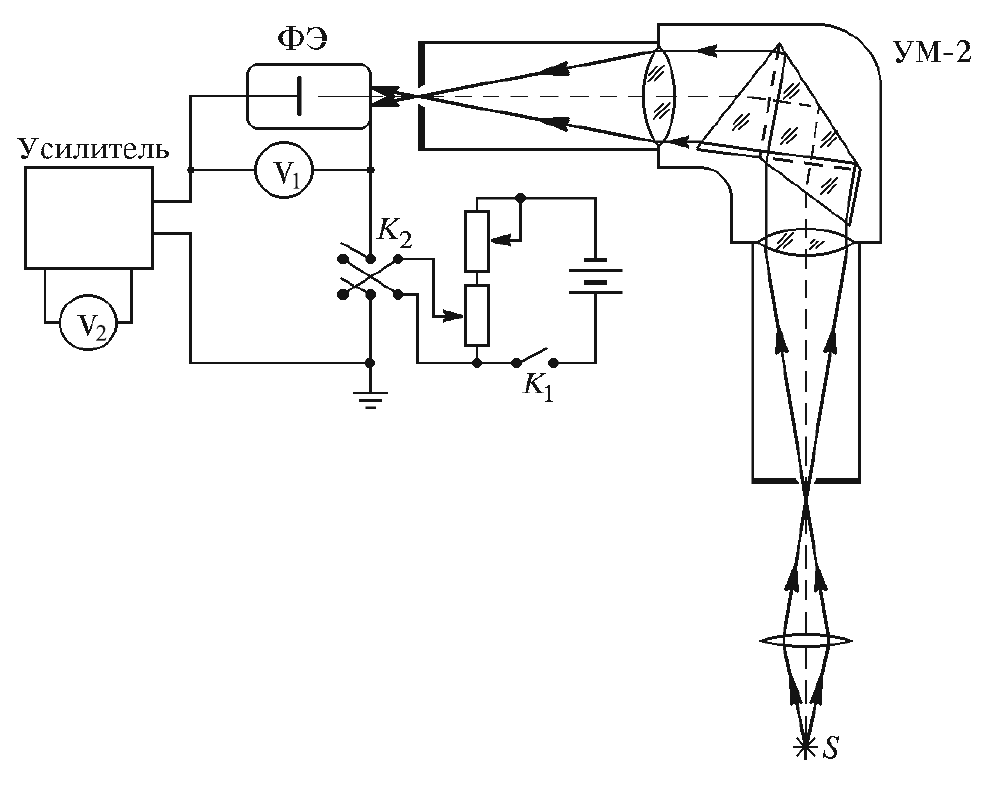
\includegraphics[width=0.9\linewidth]{res/scheme.png}
		\end{minipage}%
		\begin{minipage}{0.6\textwidth}
			\centering
			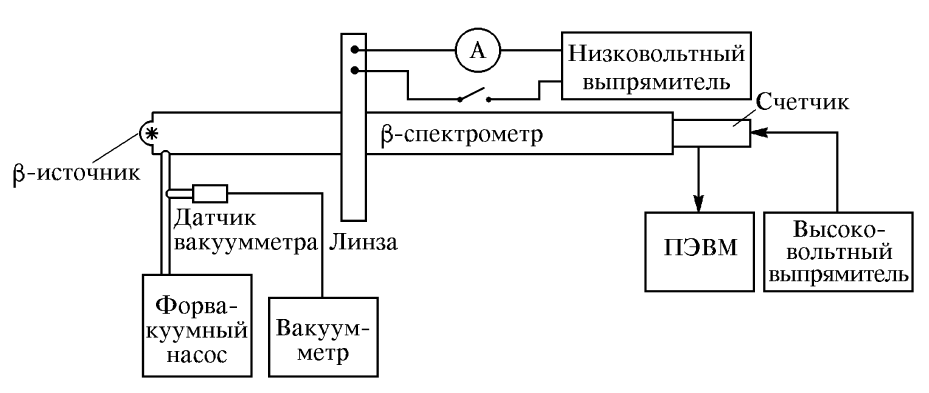
\includegraphics[width=1.0\linewidth]{photos/setup.png}
		\end{minipage}
		\caption{Схема установки для изучения фотоэффекта.}
		\label{fig:setup}
	\end{figure}
	
	В качестве источника света используется обыкновенная лампа накаливания. Свет фокусируется с помощью конденсора на входную щель монохроматора, который выделяет узкую спектральную полосу. После монохроматора свет попадает на фотокатод. Ток фотокатод-анод усиливается внутри фотоэлемента. Показания тока и потенциала запирания измеряются двумя вольтметрами.
	
	\subsection{Калибровка монохроматора}
	\begin{wrapfigure}{r}{8.0cm}
		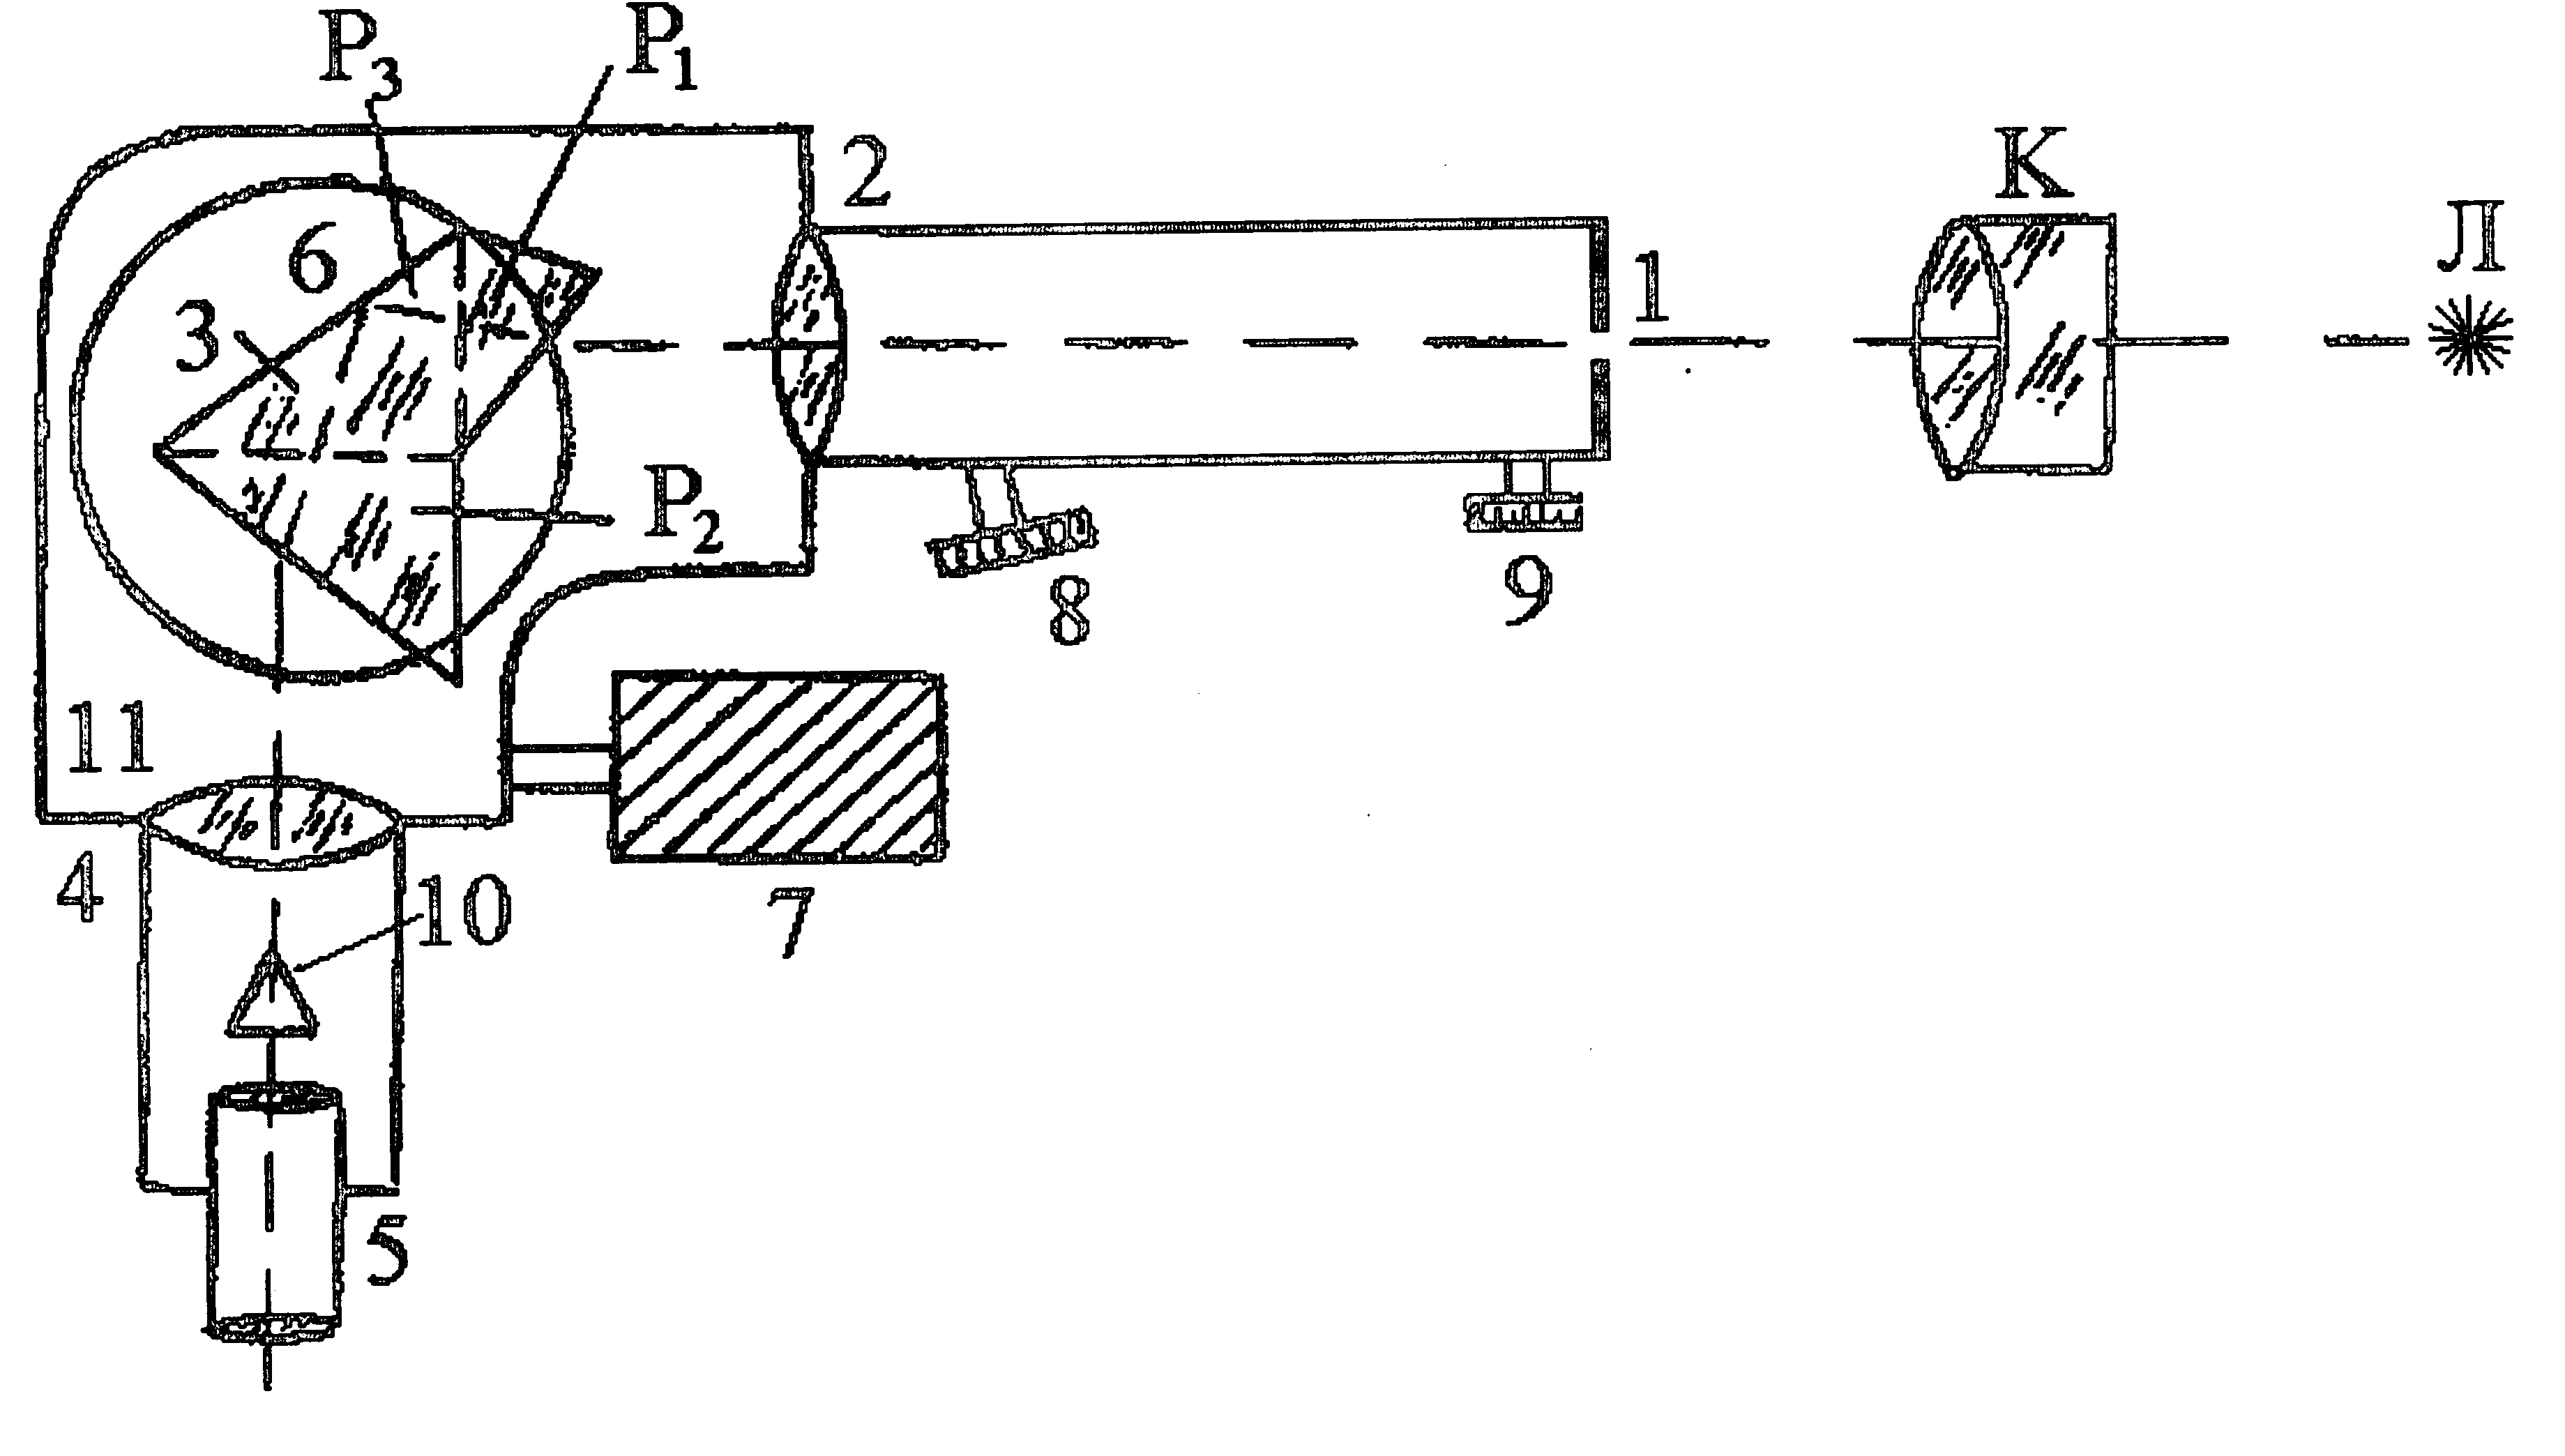
\includegraphics[width=\linewidth]{res/um2.png}
		\caption{Схема монохроматора.}
		\label{fig:monochromator}
		\vspace{-10pt}
	\end{wrapfigure}

	Спектральная линия, выделяемая монохроматором, выбирается с помощью лимба. Для проведения измерений необходима предварительная калибровка, позволяющая пересчитать показания лимба в длину волны выделяемого излучения.
	
	Для калибровки используется неоновая лампа (Л) и окуляр (5) \figref{fig:monochromator}. Неоновая лампа имеет известный дискретный спектр. Спектр наблюдается в окуляр монохроматора, установленный вместо фотоэлемента. Вращая лимб (7) можно выставить необходимую спектральную линию напротив указателя (10). Таким образом собирается набор точек $\lambda_n(N)$ и экстраполируется до зависимости $\lambda(N)$.
	
	\subsection{Фотоэлемент}
	
	\begin{wrapfigure}[10]{r}{5.0cm}
	%                  ^^ number of occupied rows
		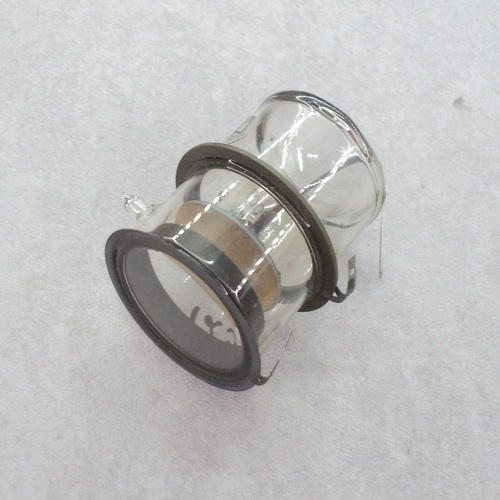
\includegraphics[width=\linewidth]{photos/f25.jpg}
		\caption{Фотоэлемент Ф25.}
		\label{fig:photoelem}
	\end{wrapfigure}
	
	Фотоэлемент представляет собой стеклянный баллон (25x30 мм), откачанный до высокого ваккума. Внутри расположен фотокатод -- тонкая пленка Na$_2$KSb(Cs), и анод, напыленный на стекло напротив фотокатода. Протекающие через фотоэлемент токи очень малы, поэтому используется усилитель постоянного тока. Усилитель смонтирован в один корпус с фотоэлементом для уменьшения наводок.
	
	Отметим, что из-за использования разных веществ проводников возникает контактная разность потенциалов. Она влияет на определение $W$ -- работы выхода, но не оказывает влияния на измерение $\hbar$ (см. формулу \ref{eq:blocking_voltage}).
	
	\newpage
	\section{Результаты}
	
	Проводим калибровку монохроматора в соответствии с методикой, описанной выше.
	
	\begin{figure}[h!]
		\centering
		\begin{minipage}{0.65\textwidth}
			\centering
			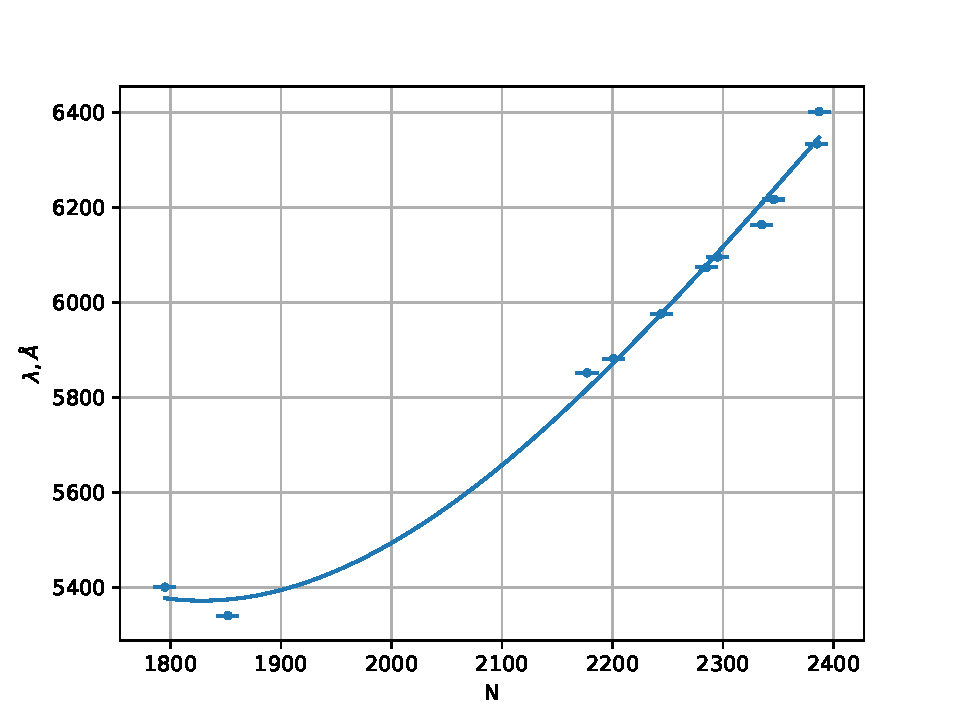
\includegraphics[width=1.0\linewidth]{gen/calibration.pdf}
		\end{minipage}
		\caption{\centering
				 Зависимость выбранной полосы неона от положения лимба.}
		\label{fig:setup}
	\end{figure}
	
	Так как нас не интересуют конкретные значения $I$ будем измерять напряжение $U_I \sim I$.
	Измеряем зависимости $U_I(V)$ для различных длин волн. Для наглядности построим графики для двух длин волн:
	
	\begin{figure}[h!]
		\centering
		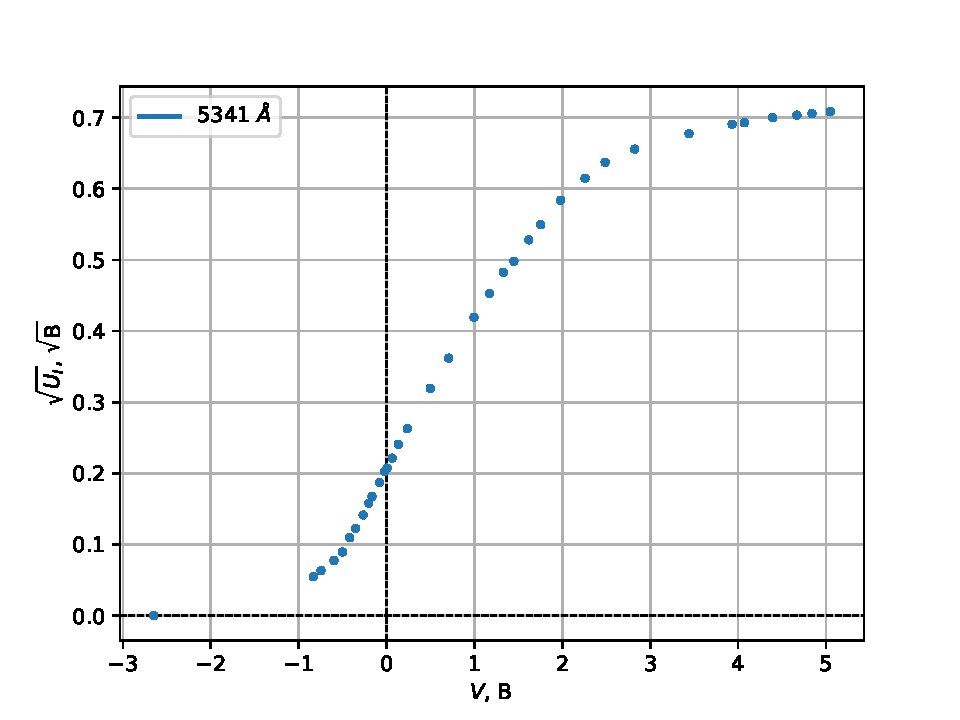
\includegraphics[width=0.7\linewidth]{gen/iv0.pdf}
		\caption{\centering
			Зависимость напряжения $U_I$ от напряжения между анодом и фотокатодом $V$.}
		\label{fig:iv_full}
	\end{figure}
	
	На графиках наблюдаются характерные особенности: напряжение запирания и насыщения.
	
	В соответствии с \eqref{eq:iv} построим линеаризацию $\sqrt{U_I}(V)$:
	
	\begin{figure}[h!]
		\centering
		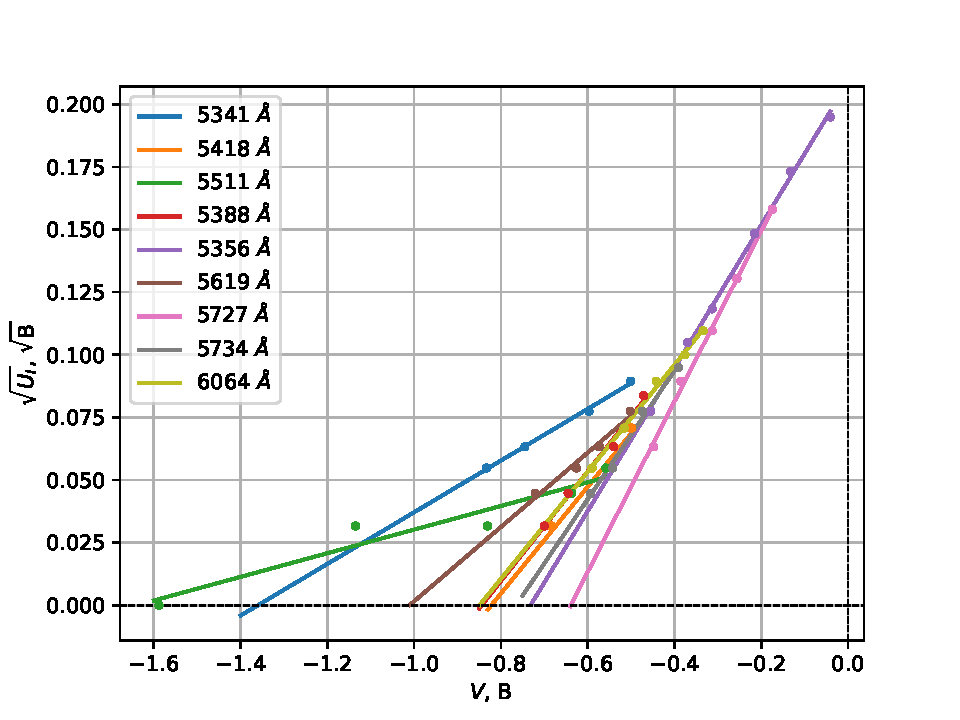
\includegraphics[width=0.8\linewidth]{gen/iv.pdf}
		\caption{\centering
				 Линеаризованная зависимость напряжения $U_I$ от напряжения между анодом и фотокатодом $V$.}
		\label{fig:iv}
	\end{figure}
	
	Из графиков определяем запирающие потенциалы $V_0$ и их погрешности.

	Построим график $V_0(\omega)$ -- запирающего напряжения от частоты света:
	
	\begin{figure}[h!]
		\centering
		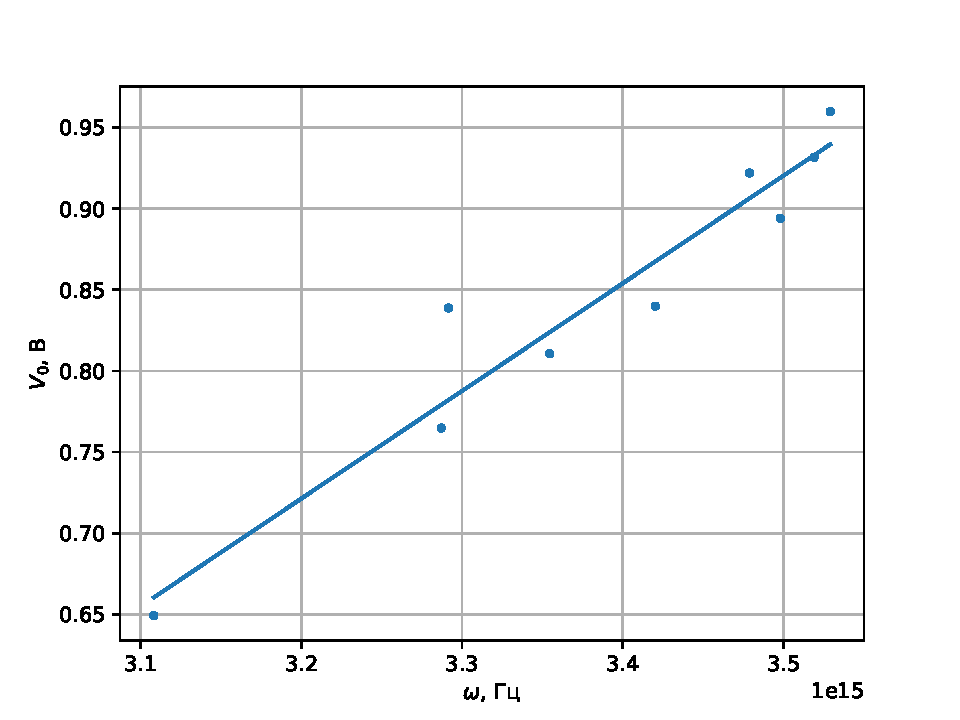
\includegraphics[width=0.8\linewidth]{gen/v0_omega.pdf}
		\caption{\centering
			Зависимость запирающего напряжения $V_0$ от частоты облучающего света $\omega$.}
		\label{fig:v0_omega}
	\end{figure}
	
	В соответствии с \eqref{eq:v0_omega} получим:
	$$\hbar = (1.06 \pm 0.12)\cdot 10^{-34} \text{ Дж}\cdot\text{с}$$
	$$W \sim 1.4 \text{ эВ}$$
	
	\section{Заключение и выводы}
	
	Данная работа подтверждает существование фотоэффекта.
	
	Получена ожидаемая зависимость \eqref{eq:iv}, подтверждено существование напряжения запирания и напряжения насыщения. Проверена зависимость напряжения запирания $V_0$ от частоты падающего на фотокатод излучения $\omega$.
	
	Получено значение постоянной Планка $\hbar = (1.06 \pm 0.12)\cdot 10^{-34} \text{ Дж}\cdot\text{с}$. Справочное значение $\hbar = 1.055\cdot 10^{-34} \text{ Дж}\cdot\text{с}$.

	Оценена работа выхода из материала фотокатода Na$_2$KSb(Cs) $W \sim 1.4 \text{ эВ}$. Из-за контактных разностей потенциалов в схеме оценка может иметь значительную систематическую погрешность.
	
		
\end{document}
\documentclass[a4paper, 12pt]{article} % тип документа

%%%Библиотеки
%\usepackage[warn]{mathtext}	
\usepackage[T2A]{fontenc}   %Кодировка
\usepackage[utf8]{inputenc} %Кодировка исходного текста
\usepackage[english, russian]{babel} %Локализация и переносы
\usepackage{caption}
\usepackage{gensymb}
%\usepackage{listings}
\usepackage{amsmath, amsfonts, amssymb, amsthm, mathtools}
%\usepackage[warn]{mathtext}
%\usepackage[mathscr]{eucal}
%\usepackage{wasysym}
\usepackage{graphicx} %Вставка картинок правильная
%\usepackage{pgfplots}
\usepackage{indentfirst}
% \usepackage{float}    %Плавающие картинки
\usepackage{wrapfig}  %Обтекание фигур (таблиц, картинок и прочего)
\usepackage{fancyhdr}  %Загрузим пакет
%\usepackage{lscape}
%\usepackage{xcolor}
%\usepackage[normalem]{ulem}
\usepackage{geometry}

\usepackage{titlesec}
\titlelabel{\thetitle.\quad}

\usepackage{hyperref}

\newgeometry{vmargin={20mm}, hmargin={25mm, 25mm}}
%%%Конец библиотек

%%%Настройка ссылок
\hypersetup
{
	colorlinks = true,
	linkcolor  = blue,
	filecolor  = magenta,
	urlcolor   = blue
}
%%%Конец настройки ссылок


%%%Настройка колонтитулы
\pagestyle{fancy}
\fancyhead{}
\fancyhead[L]{5.10.1}
\fancyhead[R]{Таранов Александр, группа Б01-206}
\fancyfoot[C]{\thepage}
%%%конец настройки колонтитулы


\begin{document}
	
	%%%Начало титульника
	\begin{titlepage}
		
		\newpage
		\begin{center}
			\normalsize Московский физико-технический институт \\(госудраственный университет)
		\end{center}
		
		\vspace{6em}
		
		\begin{center}
			\Large Лабораторная работа по общему курсу физики\\Квантовая физика
		\end{center}
		
		\vspace{1em}
		
		\begin{center}
			\Large \textbf{Фотоэффект.}
		\end{center}
		
		\vspace{2em}
		
		\begin{center}
			\large Таранов Александр, На подсосе: Владислав Костылев \\
			Группа Б01-206
		\end{center}
		
		\vspace{\fill}
		
	\end{titlepage}
	%%%Конец Титульника
	
	
	
	%%%Настройка оглавления и нумерации страниц
	\thispagestyle{empty}
	\newpage
	\tableofcontents
	\newpage
	\setcounter{page}{1}
	%%%Настройка оглавления и нумерации страниц

	\section{Теоретическое введение}
	
	\subsection{Базовые принципы фотоэффекта}
	
	Подвергая поверхность фотокатода освещению можно обнаружить испускание электронов с поверхности катода. Данное явление называется одноквантовым фотоэлектрическим эффектом.
	Свойства фотоэффекта не имеют объяснения в рамках классической физики, но их обоснование существует в рамках квантовой физики. Для этого используется модель квантов света -- фотонов.
	
	Рассмотрим случай монохроматического излучения частотой $\omega$. При взаимодействии фотона с электроном в веществе фотон может полностью поглотиться, передав энергию электрону:
	
	\begin{equation}
		\hbar \omega = E_{max} + W,
		\label{eq:basic}
	\end{equation}
	где $W$ -- работа выхода, $E_{max}$ -- максимальная энергия, которую может приобрести электрон. 
	
	\subsection{Фотэффект в металле}

	Рассмотрим распределение фотоэлектронов по энергии в металле.
	
	Как известно, электроны в металлах могут легко перемещаться под действием электрического поля. Эти электроны являются валентными электронами металла; они слабо связаны с кристаллической решеткой. Поведение этих свободных электронов хорошо описывается моделью идеального газа.
	
	Электроны являются фермионами, имея спин $+\frac{1}{2}$. Фермионы подчиняются принципу Паули: на одно квантовое состояние приходится не более двух фермионов с противоположными спинами. Из этого следует, что в потенциальной яме, образованной металлом, все электроны не могут расположиться на дне $E = 0$: они распределятся по разрешенным уровням до некоторой энергии $E_F$ -- \textit{энергии Ферми} (см. \ref{fig:metal}). Образуется \textit{зона проводимости}.
	
	Энергия Ферми определяется концентрацией и составляет $(1\div10)$ эВ, намного превышая тепловую энергию электронов $\approx 25$ мэВ. Поэтому влиянием температурных явлений можно пренебречь.
	
	Для выхода электрону необходимо преодолеть притяжение к металлу -- совершить \textit{работу выхода}. Ее можно оценить как работу по разнесению электрона и его "изображения" на бесконечное расстояние: $W = \frac{e^2}{r_0}$.
	
	\begin{figure}[h!]
		\centering
		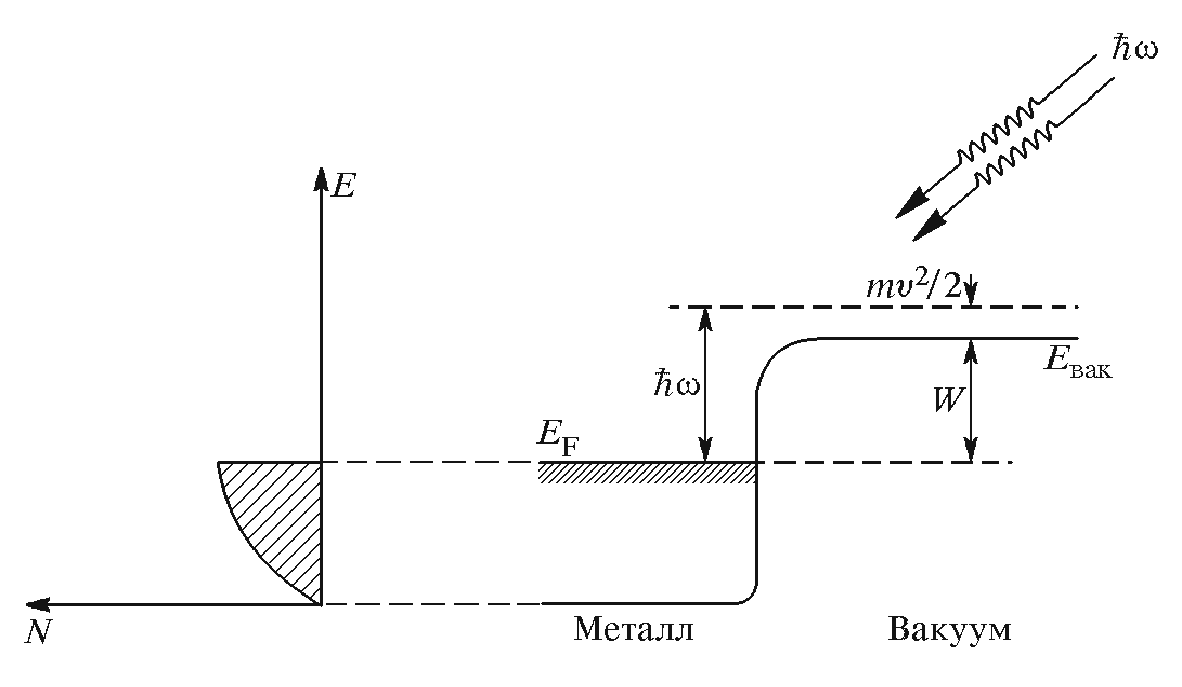
\includegraphics[scale=0.5]{res/metal.png}
		\caption{\centering
				 Модель металла как потенциальной ямы с электронным газом.
				 Слева от оси энергий: распределение электронов по энергиям.
				 Справа от оси энергий: схема зон.}
		\label{fig:metal}
	\end{figure}
	
	Таким образом, для выхода электрона из металла нужно совершить работу выхода $W$, равную разности потенциальной энергии электрона в вакууме $E_{\text{вак}}$ и энергии Ферми $E_F$. При этом фотоны, имеющие энергию $E > W$ могут выбивать электроны с более глубоких уровней. Этим объясняется распределение энергии электронов при фотоэффекте. Отметим, что квантовый выход металлов $\frac{N_{\text{электронов}}}{N_{\text{фотонов}}}$ мал, поскольку большая часть фотонов отражается.

\newpage

\subsection{Фотоэффект в полупроводниках}
	\begin{wrapfigure}[17]{l}{7.0cm}
	%                  ^^ number of occupied rows
		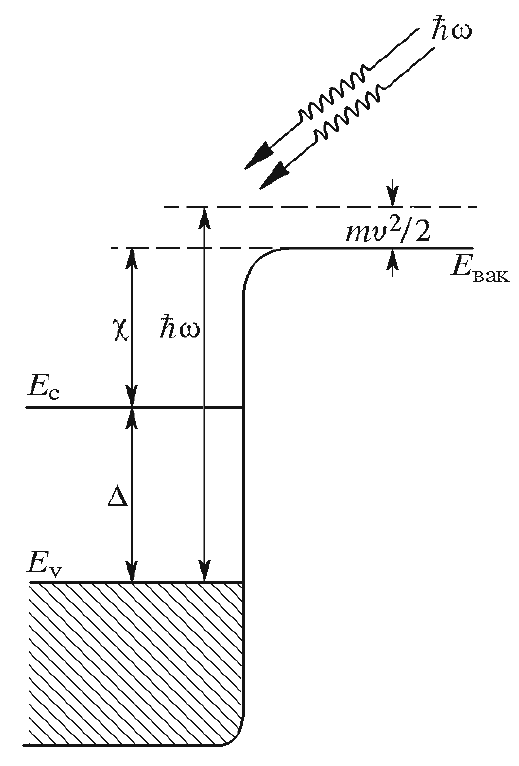
\includegraphics[scale=0.6]{res/semiconductor.png}
		% \caption{Модель полупроводника как потенциальной ямы.}
		\label{fig:semiconductor}
		\vspace{0pt}
	\end{wrapfigure}
	
	Схема зон в полупроводниках и металлах сильно различаются. В полупроводнике при абсолютном нуле валентные электроны полностью заполняют \textit{валентную зону}. Особенностью полупроводников является \textit{запрещенная зона}, которая отделяет валентную зону от зоны проводимости. Этим объясняется низкая проводимость полупроводников: проводящими являются электроны, которые попали в проводящую зону за счет тепло- или фотовозбуждения.
	
	Принципиальное описание фотоэффекта аналогично фотоэффекту в металлах, выполняется соотношение Эйнштейна: 
	
	\begin{center}
		$\hbar \omega = \Delta + \chi + E_{max}$.
	\end{center}
	
	На рис. \ref{fig:semiconductor} приведены основные обозначения, используемые для описания зон полупроводника.
	
	\begin{itemize}
		\item $E_v$ -- потолок валентной зоны,
		\item $E_c$ -- дно зоны проводимости,
		\item $E_c - E_v = \Delta$ -- ширина запрещенной зоны,
		\item $E_{\text{вак}} - E_c = \chi$ -- электронное сродство.
	\end{itemize}
	
	\newpage
		
	\subsection{Измерение энергии электронов}
	\begin{wrapfigure}{r}{7.0cm}
		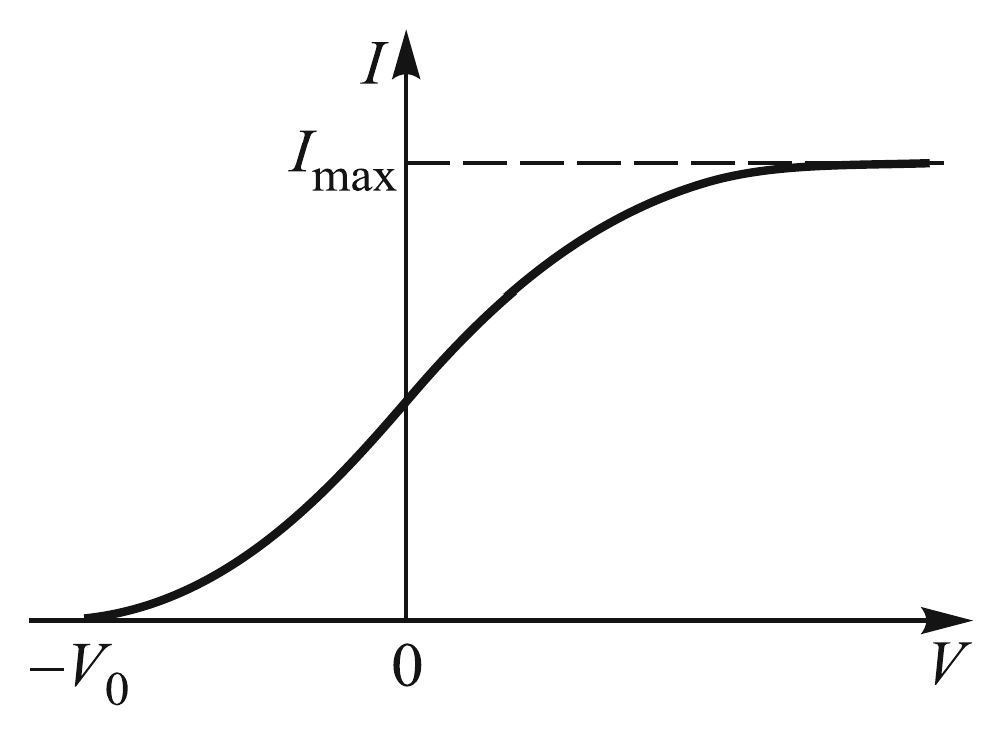
\includegraphics[scale=0.3]{res/iv_curve.png}
		\caption{ВАХ для пары фотокатод-анод.}
		\label{fig:iv_curve}
		\vspace{-10pt}
	\end{wrapfigure}

	Для измерения энергии фотоэлектронов используются пара фотокатод-анод. Между ними создается \textit{ускоряющий} $(V < 0)$ или \textit{задерживающий} $(V > 0)$ потенциал.
	
	При увеличениии напряжения $V$ фототок достигает насыщения: все фотоэлектроны достигают анода. При уменьшении напряжения существует точка $V = -V_0$  в отрицательной области напряжений, где фототок обнуляется: даже самые высокоэнергетичные электроны не могут преодолеть барьер. $V_0$ называется \textit{потенциалом запирания}.
	
	Таким образом, мы можем модифицировать \eqref{eq:basic}:
	\begin{equation}
		e V_0 = \hbar \omega - W.
		\label{eq:blocking_voltage}
	\end{equation}
	
	Если бы фотокатод был очень тонким ($\sim 10$ \AA), зависимость \figref{fig:iv_curve} имела бы скачок возле $eV_0 = h\omega - W$, так как почти все электроны бы имели одинаковые кинетические энергии. Но фотокатод имеет $10^2 \div 10^3$ атомных слоев в толщину, что видоизменяет зависимость на плавную.
	
	В опыте ВАХ экстраполируется к нулевому току для оценки запирающего потенциала $V_0$. Расчет для геометрии плоских параллельных анода и фотокатода дает 
	\begin{equation}
		\sqrt{I} \propto (V_0 - V).
		\label{eq:iv}
	\end{equation}
	
	В работе опыты проводятся для различных частот $\omega$. Из экстраполированных потенциалов запирания строится зависимость $V_0(\omega)$. В соответствии с \eqref{eq:blocking_voltage}:
	\begin{equation}
		V_0(\omega) = \frac{\hbar\omega - W}{e}
		\label{eq:v0_omega}
	\end{equation}
	
	Из графика $V_0(\omega)$ можно определить постоянную Планка $\hbar$ и работу выхода $W$.
	
	\section{Методика эксперимента}
	
	\begin{figure}[h!]
		\centering
		\begin{minipage}{0.4\textwidth}
			\centering
			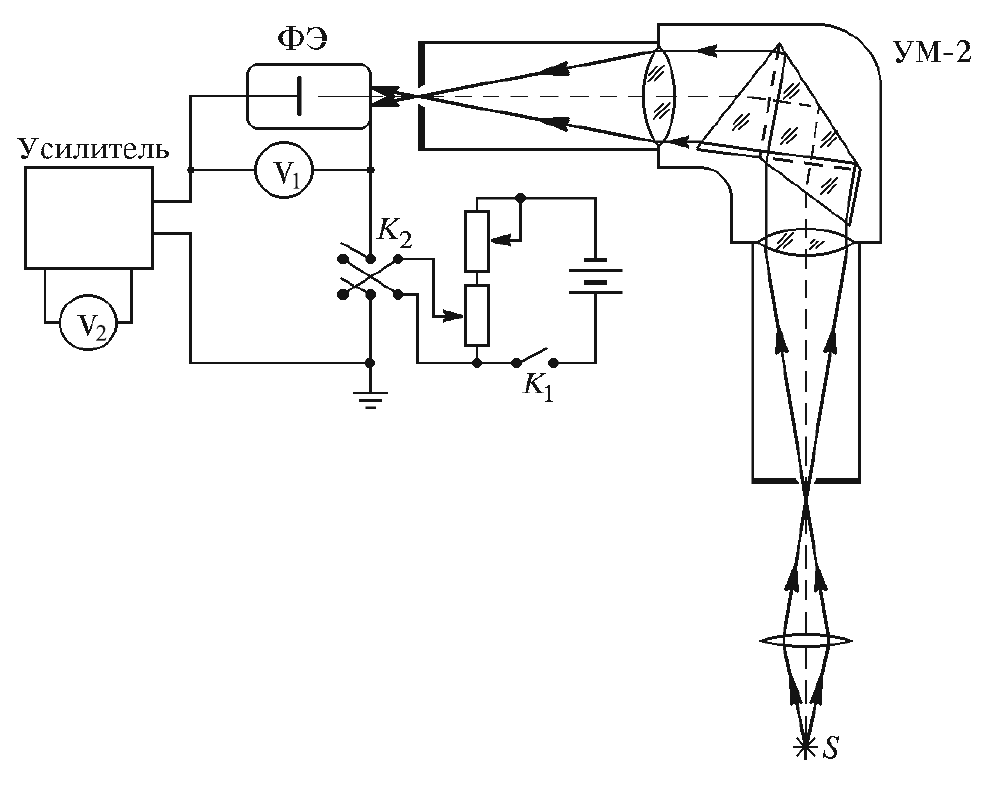
\includegraphics[width=0.9\linewidth]{res/scheme.png}
		\end{minipage}%
		\begin{minipage}{0.6\textwidth}
			\centering
			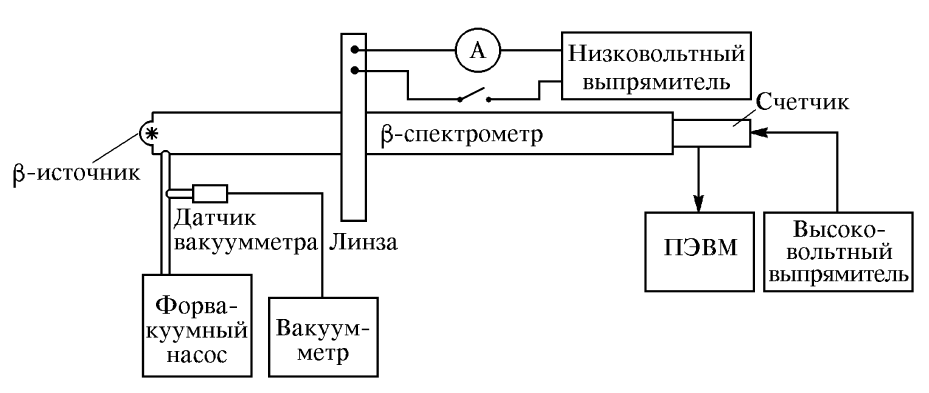
\includegraphics[width=1.0\linewidth]{photos/setup.png}
		\end{minipage}
		\caption{Схема установки для изучения фотоэффекта.}
		\label{fig:setup}
	\end{figure}
	
	В качестве источника света используется обыкновенная лампа накаливания. Свет фокусируется с помощью конденсора на входную щель монохроматора, который выделяет узкую спектральную полосу. После монохроматора свет попадает на фотокатод. Ток фотокатод-анод усиливается внутри фотоэлемента. Показания тока и потенциала запирания измеряются двумя вольтметрами.
	
	\subsection{Калибровка монохроматора}
	\begin{wrapfigure}{r}{8.0cm}
		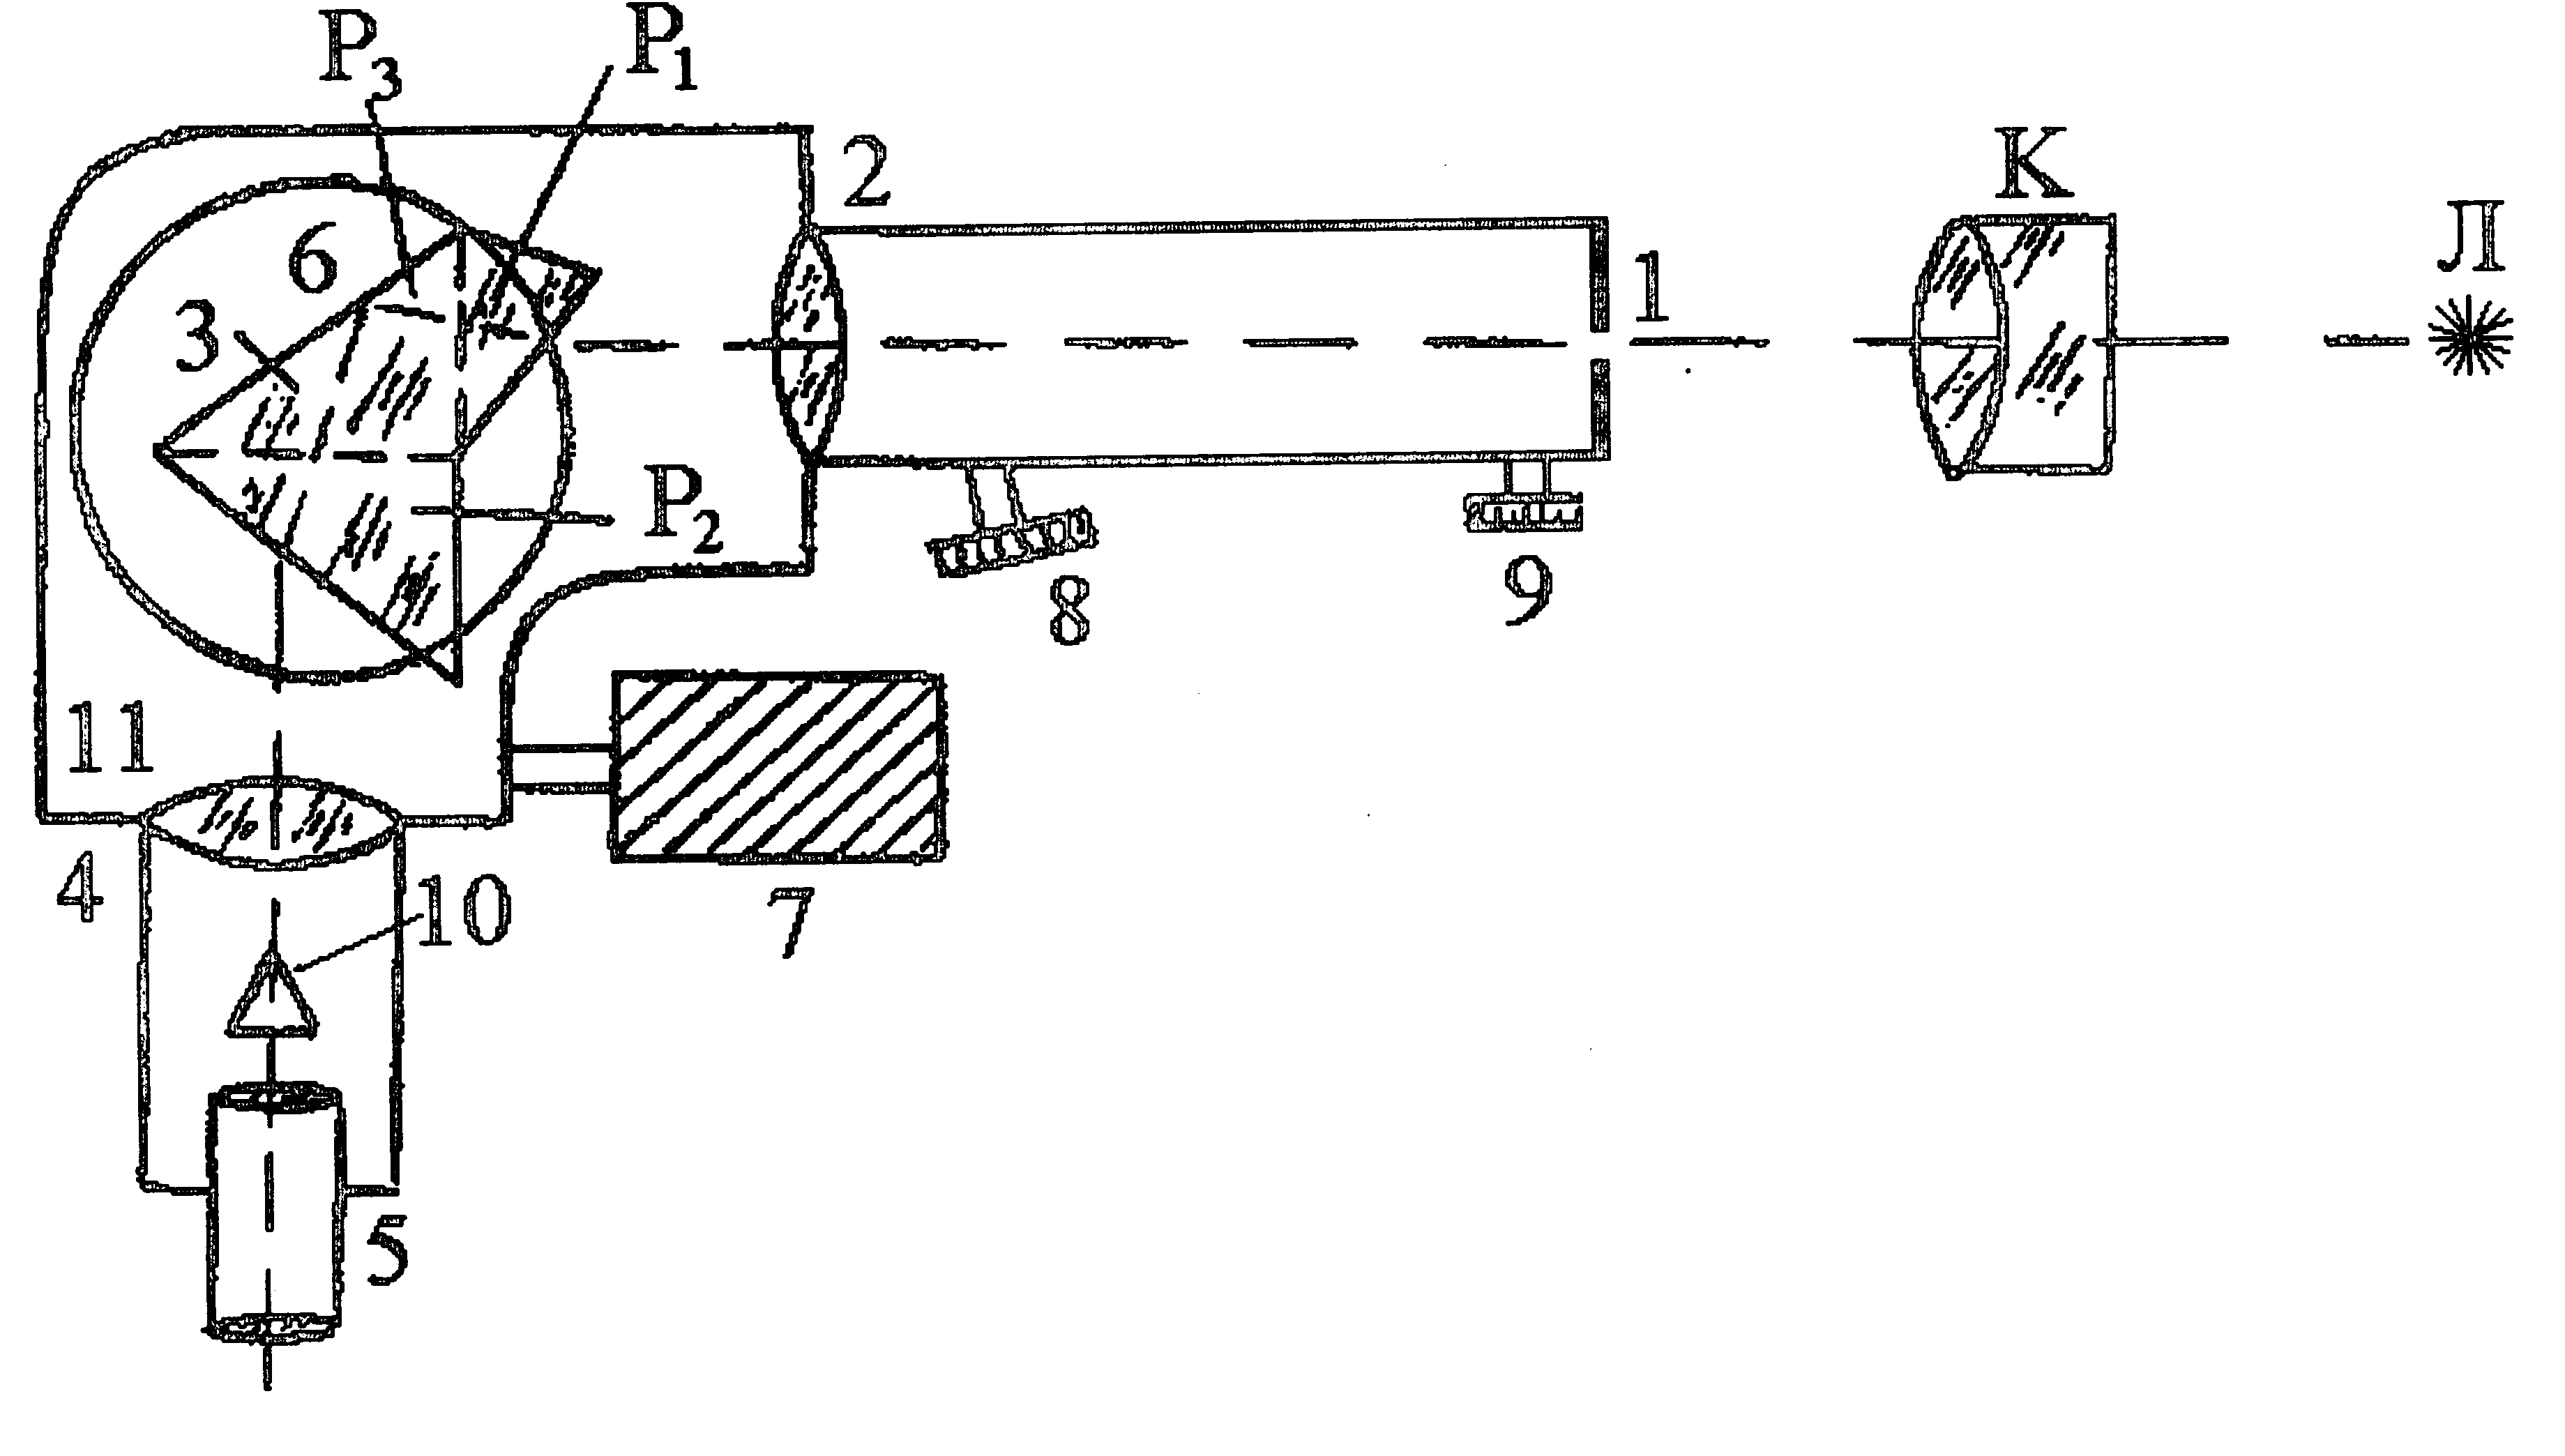
\includegraphics[width=\linewidth]{res/um2.png}
		\caption{Схема монохроматора.}
		\label{fig:monochromator}
		\vspace{-10pt}
	\end{wrapfigure}

	Спектральная линия, выделяемая монохроматором, выбирается с помощью лимба. Для проведения измерений необходима предварительная калибровка, позволяющая пересчитать показания лимба в длину волны выделяемого излучения.
	
	Для калибровки используется неоновая лампа (Л) и окуляр (5) \figref{fig:monochromator}. Неоновая лампа имеет известный дискретный спектр. Спектр наблюдается в окуляр монохроматора, установленный вместо фотоэлемента. Вращая лимб (7) можно выставить необходимую спектральную линию напротив указателя (10). Таким образом собирается набор точек $\lambda_n(N)$ и экстраполируется до зависимости $\lambda(N)$.
	
	\subsection{Фотоэлемент}
	
	\begin{wrapfigure}[10]{r}{5.0cm}
	%                  ^^ number of occupied rows
		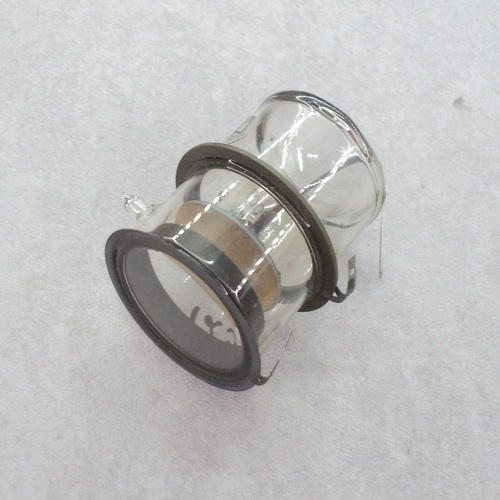
\includegraphics[width=\linewidth]{photos/f25.jpg}
		\caption{Фотоэлемент Ф25.}
		\label{fig:photoelem}
	\end{wrapfigure}
	
	Фотоэлемент представляет собой стеклянный баллон (25x30 мм), откачанный до высокого ваккума. Внутри расположен фотокатод -- тонкая пленка Na$_2$KSb(Cs), и анод, напыленный на стекло напротив фотокатода. Протекающие через фотоэлемент токи очень малы, поэтому используется усилитель постоянного тока. Усилитель смонтирован в один корпус с фотоэлементом для уменьшения наводок.
	
	Отметим, что из-за использования разных веществ проводников возникает контактная разность потенциалов. Она влияет на определение $W$ -- работы выхода, но не оказывает влияния на измерение $\hbar$ (см. формулу \ref{eq:blocking_voltage}).
	
	\newpage
	\section{Результаты}
	
	Проводим калибровку монохроматора в соответствии с методикой, описанной выше.
	
	\begin{figure}[h!]
		\centering
		\begin{minipage}{0.65\textwidth}
			\centering
			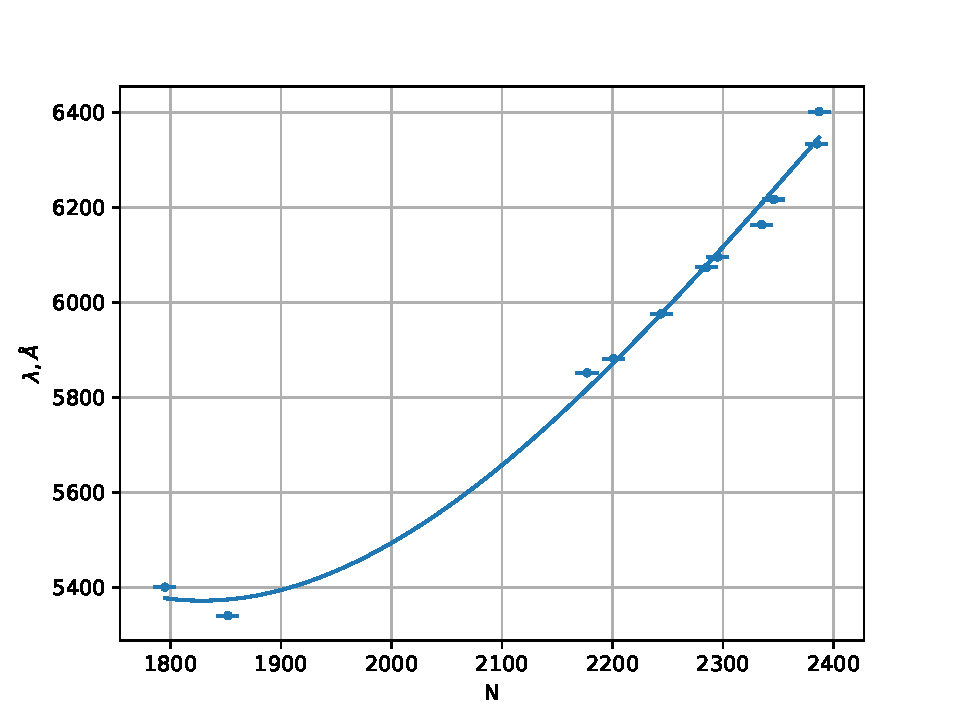
\includegraphics[width=1.0\linewidth]{gen/calibration.pdf}
		\end{minipage}
		\caption{\centering
				 Зависимость выбранной полосы неона от положения лимба.}
		\label{fig:setup}
	\end{figure}
	
	Так как нас не интересуют конкретные значения $I$ будем измерять напряжение $U_I \sim I$.
	Измеряем зависимости $U_I(V)$ для различных длин волн. Для наглядности построим графики для двух длин волн:
	
	\begin{figure}[h!]
		\centering
		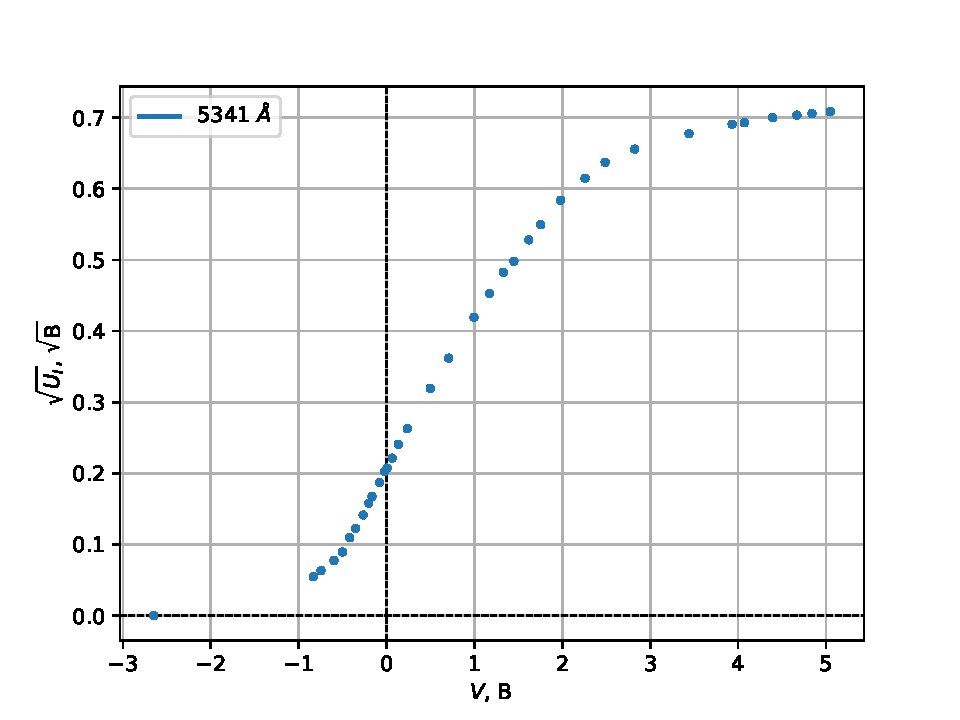
\includegraphics[width=0.7\linewidth]{gen/iv0.pdf}
		\caption{\centering
			Зависимость напряжения $U_I$ от напряжения между анодом и фотокатодом $V$.}
		\label{fig:iv_full}
	\end{figure}
	
	На графиках наблюдаются характерные особенности: напряжение запирания и насыщения.
	
	В соответствии с \eqref{eq:iv} построим линеаризацию $\sqrt{U_I}(V)$:
	
	\begin{figure}[h!]
		\centering
		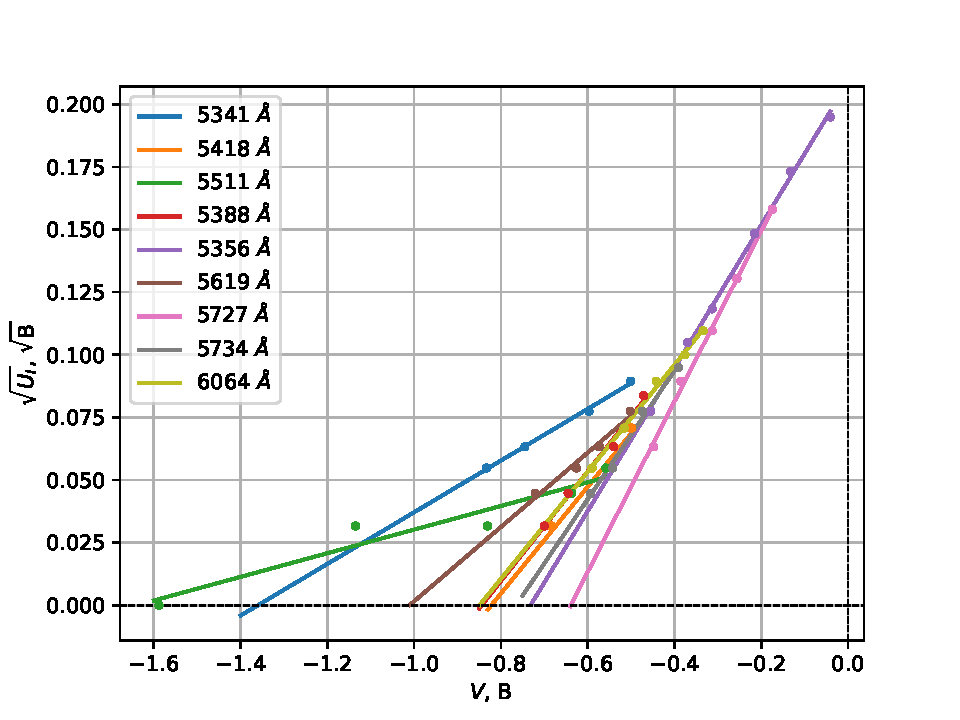
\includegraphics[width=0.8\linewidth]{gen/iv.pdf}
		\caption{\centering
				 Линеаризованная зависимость напряжения $U_I$ от напряжения между анодом и фотокатодом $V$.}
		\label{fig:iv}
	\end{figure}
	
	Из графиков определяем запирающие потенциалы $V_0$ и их погрешности.

	Построим график $V_0(\omega)$ -- запирающего напряжения от частоты света:
	
	\begin{figure}[h!]
		\centering
		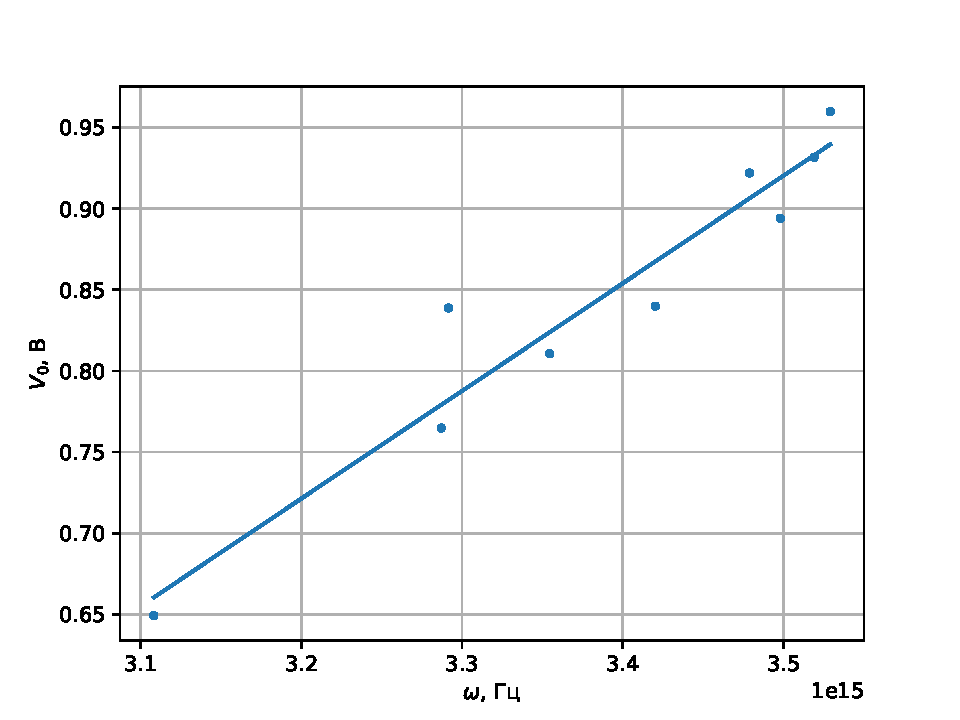
\includegraphics[width=0.8\linewidth]{gen/v0_omega.pdf}
		\caption{\centering
			Зависимость запирающего напряжения $V_0$ от частоты облучающего света $\omega$.}
		\label{fig:v0_omega}
	\end{figure}
	
	В соответствии с \eqref{eq:v0_omega} получим:
	$$\hbar = (1.06 \pm 0.12)\cdot 10^{-34} \text{ Дж}\cdot\text{с}$$
	$$W \sim 1.4 \text{ эВ}$$
	
	\section{Заключение и выводы}
	
	Данная работа подтверждает существование фотоэффекта.
	
	Получена ожидаемая зависимость \eqref{eq:iv}, подтверждено существование напряжения запирания и напряжения насыщения. Проверена зависимость напряжения запирания $V_0$ от частоты падающего на фотокатод излучения $\omega$.
	
	Получено значение постоянной Планка $\hbar = (1.06 \pm 0.12)\cdot 10^{-34} \text{ Дж}\cdot\text{с}$. Справочное значение $\hbar = 1.055\cdot 10^{-34} \text{ Дж}\cdot\text{с}$.

	Оценена работа выхода из материала фотокатода Na$_2$KSb(Cs) $W \sim 1.4 \text{ эВ}$. Из-за контактных разностей потенциалов в схеме оценка может иметь значительную систематическую погрешность.
	
		
\end{document}

